\tikzset{every picture/.style={line width=0.75pt}}

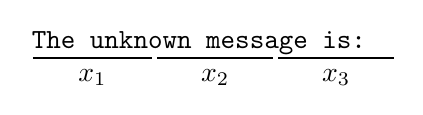
\begin{tikzpicture}[x=0.75pt,y=0.75pt,yscale=-1,xscale=1]


\draw    (4,17) -- (61.5,17) ;
\draw    (64,17) -- (119.7,17) ;
\draw    (122.3,17) -- (178,17) ;

\draw (2,3) node [anchor=north west][inner sep=0.75pt]   [align=left] {
\texttt{The unknown message is:}
};

\draw (32.75,21) node [anchor=north] [inner sep=0.75pt]    {$x_{1}$};
\draw (91.85,21) node [anchor=north] [inner sep=0.75pt]    {$x_{2}$};
\draw (150.15,21) node [anchor=north] [inner sep=0.75pt]    {$x_{3}$};

\end{tikzpicture}